\chapter{Validación}

\section{Programando con facetas públicas}
Poseer un sistema de inferencia en conjunto con un plugin para IDEs tiene múltiples beneficios. Primero, evita la anotación de facetas públicas en identificadores no relevantes para el análisis. Segundo, provee comodidad al momento de programar, ya que se obtienen en tiempo real los resultados de la inferencia, sin tener que re-ejecutar un análisis. Por último, aumenta la escalabilidad de los sistemas, ya que el costo de refactorizar código anotado es mayor al costo de refactorizar código no anotado.

A continuación, se muestran algunas capturas de pantalla que ejemplifican la interacción entre el plugin y el programador.

La figura \ref{screen1} ilustra la integración de los errores del plugin con los errores de Dart, en la misma ventana del IDE.

\begin{figure}[ht]
  \centering
  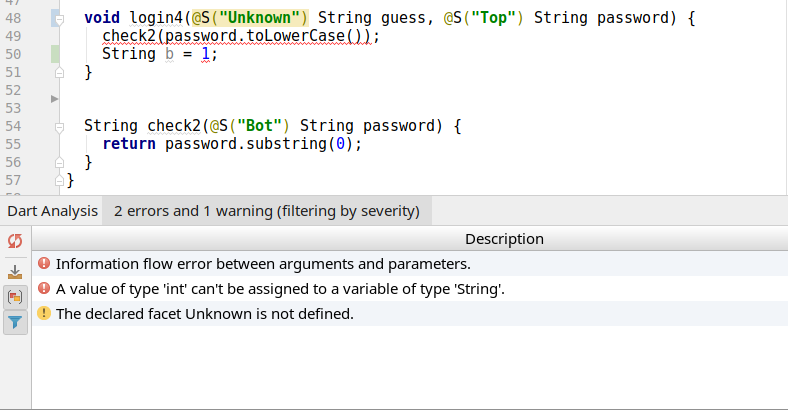
\includegraphics[width=0.8\textwidth]{imagenes/screen1.png}
  \caption{Errores integrados con errores de Dart}
  \label{screen1}
\end{figure}
\clearpage

La figura \ref{screen2} muestra la información inferida al ubicar el cursor sobre un identificador sin faceta pública declarada.

\begin{figure}[ht]
  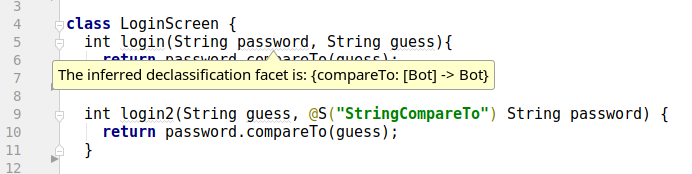
\includegraphics[width=\textwidth]{imagenes/facetinfo.png}
  \caption{Faceta pública inferida}
  \label{screen2}
\end{figure}


La figura \ref{screen3} muestra un error generado por un flujo no permitido.

\begin{figure}[ht]
  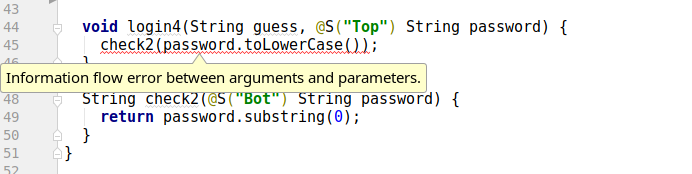
\includegraphics[width=\textwidth]{imagenes/flow.png}
  \caption{Error de flujo de información}
  \label{screen3}
\end{figure}

La figura \ref{screen4} muestra un error generado por la declaración de una faceta pública no definida.

\begin{figure}[ht]
  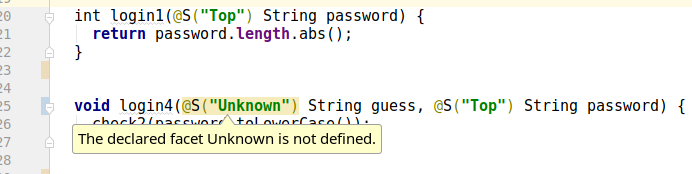
\includegraphics[width=\textwidth]{imagenes/undefined.png}
  \caption{Warning ante faceta pública no definida}
  \label{screen4}
\end{figure}
\clearpage
La figura \ref{screen5} muestra un identificador cuya faceta pública no pudo ser inferida con precisión, debido a que cualquier faceta genera un programa bien tipado.

\begin{figure}[ht]
  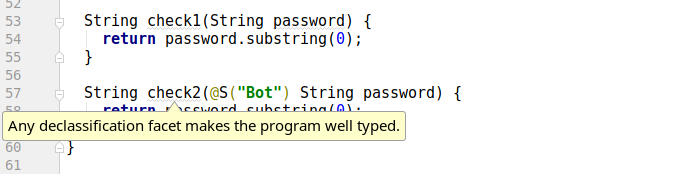
\includegraphics[width=\textwidth]{imagenes/any.png}
  \caption{Toda faceta pública genera un programa bien tipado}
  \label{screen5}
\end{figure}

\section{Batería de tests}
En conjunto con uno de los autores de type-based declassification, se validaron una serie de tests unitarios que ponen a prueba el cumplimiento de las reglas del sistema de tipos.

Además de proveer una forma de validación de este trabajo, los tests unitarios sirvieron como guía para la implementación de las distintas componentes.

Para escribir los tests se utilizó la librería estándar de testing en Dart.

\section{Repositorio de prueba}
Para demostrar el uso del análisis en un ejemplo realista, se creó un pequeño sistema de login web, programado con facetas públicas de type-based declassification. El código se encuentra en un repositorio de GitHub~\cite{repotest}.

En este ejemplo se pudo constatar la utilidad del sistema de inferencia. De las 20 declaraciones de identificadores del código, solo 6 de ellas fueron anotadas con facetas públicas, y el resto fue inferido de acuerdo a las reglas del sistema de tipos.
